% Generated by AP Math GOLD PILOT deterministic Python generator.
% input id: 06_function_tangent_triple_root
\documentclass{article}
\usepackage[margin=1cm]{geometry}
\def\pgfsysdriver{pgfsys-dvisvgm.def}
\usepackage{fontspec}
\setmainfont{Malgun Gothic}
\setsansfont{Malgun Gothic}
\usepackage{amsmath}
\usepackage{amssymb}
\usepackage{pgfplots}
\pgfplotsset{compat=1.18}
\pagestyle{empty}
\begin{document}
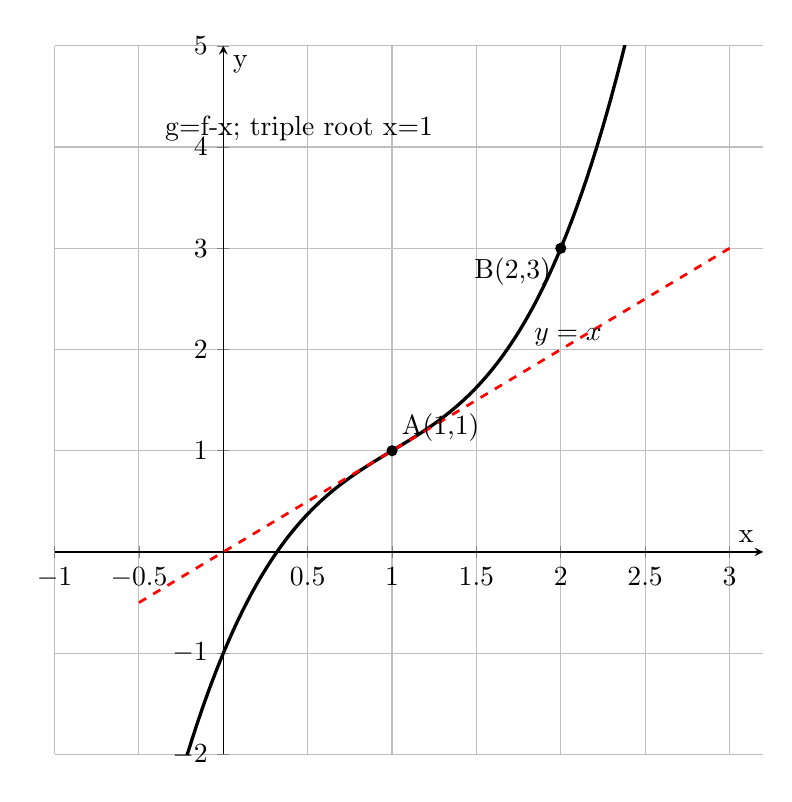
\begin{tikzpicture}
\begin{axis}[width=9cm,height=9cm,scale only axis,axis lines=middle,grid=major,xmin=-1,xmax=3.2,ymin=-2,ymax=5,xlabel={x},ylabel={y},clip=true]
\addplot[black, solid, line width=1.2pt] coordinates {(-0.5,-3.875) (-0.470833,-3.652762) (-0.441667,-3.438031) (-0.4125,-3.230658) (-0.383333,-3.030495) (-0.354167,-2.837393) (-0.325,-2.651203) (-0.295833,-2.471776) (-0.266667,-2.298963) (-0.2375,-2.132615) (-0.208333,-1.972584) (-0.179167,-1.81872) (-0.15,-1.670875) (-0.120833,-1.5289) (-0.091667,-1.392645) (-0.0625,-1.261963) (-0.033333,-1.136704) (-0.004167,-1.016719) (0.025,-0.901859) (0.054167,-0.791976) (0.083333,-0.686921) (0.1125,-0.586545) (0.141667,-0.490698) (0.170833,-0.399233) (0.2,-0.312) (0.229167,-0.22885) (0.258333,-0.149635) (0.2875,-0.074205) (0.316667,-0.002412) (0.345833,0.065893) (0.375,0.130859) (0.404167,0.192635) (0.433333,0.25137) (0.4625,0.307213) (0.491667,0.360312) (0.520833,0.410816) (0.55,0.458875) (0.579167,0.504637) (0.608333,0.548251) (0.6375,0.589865) (0.666667,0.62963) (0.695833,0.667693) (0.725,0.704203) (0.754167,0.73931) (0.783333,0.773162) (0.8125,0.805908) (0.841667,0.837697) (0.870833,0.868678) (0.9,0.899) (0.929167,0.928811) (0.958333,0.958261) (0.9875,0.987498) (1.016667,1.016671) (1.045833,1.04593) (1.075,1.075422) (1.104167,1.105297) (1.133333,1.135704) (1.1625,1.166791) (1.191667,1.198708) (1.220833,1.231603) (1.25,1.265625) (1.279167,1.300923) (1.308333,1.337646) (1.3375,1.375943) (1.366667,1.415963) (1.395833,1.457854) (1.425,1.501766) (1.454167,1.547846) (1.483333,1.596245) (1.5125,1.647111) (1.541667,1.700593) (1.570833,1.75684) (1.6,1.816) (1.629167,1.878223) (1.658333,1.943657) (1.6875,2.012451) (1.716667,2.084755) (1.745833,2.160716) (1.775,2.240484) (1.804167,2.324208) (1.833333,2.412037) (1.8625,2.504119) (1.891667,2.600604) (1.920833,2.701639) (1.95,2.807375) (1.979167,2.91796) (2.008333,3.033542) (2.0375,3.154271) (2.066667,3.280296) (2.095833,3.411766) (2.125,3.548828) (2.154167,3.691633) (2.183333,3.840329) (2.2125,3.995064) (2.241667,4.155989) (2.270833,4.323251) (2.3,4.497) (2.329167,4.677384) (2.358333,4.864553) (2.3875,5.058654) (2.416667,5.259838) (2.445833,5.468253) (2.475,5.684047) (2.504167,5.90737) (2.533333,6.13837) (2.5625,6.377197) (2.591667,6.623999) (2.620833,6.878926) (2.65,7.142125) (2.679167,7.413746) (2.708333,7.693938) (2.7375,7.98285) (2.766667,8.28063) (2.795833,8.587427) (2.825,8.903391) (2.854167,9.228669) (2.883333,9.563412) (2.9125,9.907768) (2.941667,10.261885) (2.970833,10.625913) (3,11)};
\node[anchor=west] at (axis cs:3,11) {$f(x)$};
\addplot[red, dashed, line width=1pt] coordinates {(-0.5,-0.5) (-0.45625,-0.45625) (-0.4125,-0.4125) (-0.36875,-0.36875) (-0.325,-0.325) (-0.28125,-0.28125) (-0.2375,-0.2375) (-0.19375,-0.19375) (-0.15,-0.15) (-0.10625,-0.10625) (-0.0625,-0.0625) (-0.01875,-0.01875) (0.025,0.025) (0.06875,0.06875) (0.1125,0.1125) (0.15625,0.15625) (0.2,0.2) (0.24375,0.24375) (0.2875,0.2875) (0.33125,0.33125) (0.375,0.375) (0.41875,0.41875) (0.4625,0.4625) (0.50625,0.50625) (0.55,0.55) (0.59375,0.59375) (0.6375,0.6375) (0.68125,0.68125) (0.725,0.725) (0.76875,0.76875) (0.8125,0.8125) (0.85625,0.85625) (0.9,0.9) (0.94375,0.94375) (0.9875,0.9875) (1.03125,1.03125) (1.075,1.075) (1.11875,1.11875) (1.1625,1.1625) (1.20625,1.20625) (1.25,1.25) (1.29375,1.29375) (1.3375,1.3375) (1.38125,1.38125) (1.425,1.425) (1.46875,1.46875) (1.5125,1.5125) (1.55625,1.55625) (1.6,1.6) (1.64375,1.64375) (1.6875,1.6875) (1.73125,1.73125) (1.775,1.775) (1.81875,1.81875) (1.8625,1.8625) (1.90625,1.90625) (1.95,1.95) (1.99375,1.99375) (2.0375,2.0375) (2.08125,2.08125) (2.125,2.125) (2.16875,2.16875) (2.2125,2.2125) (2.25625,2.25625) (2.3,2.3) (2.34375,2.34375) (2.3875,2.3875) (2.43125,2.43125) (2.475,2.475) (2.51875,2.51875) (2.5625,2.5625) (2.60625,2.60625) (2.65,2.65) (2.69375,2.69375) (2.7375,2.7375) (2.78125,2.78125) (2.825,2.825) (2.86875,2.86875) (2.9125,2.9125) (2.95625,2.95625) (3,3)};
% verified tangent: yx / f
\addplot[only marks,mark=*,mark size=1.8pt,black] coordinates {(1,1)};
\addplot[only marks,mark=*,mark size=1.8pt,black] coordinates {(2,3)};
\node[anchor=south west] at (axis cs:1,1) {A(1,1)};
\node[anchor=north east] at (axis cs:2,3) {B(2,3)};
\node[anchor=north east] at (axis cs:2.3,2.3) {$y=x$};
\node[anchor=north east] at (axis cs:1.3,4.4) {g=f-x; triple root x=1};
\end{axis}
\end{tikzpicture}
\end{document}
